%%%%%%%%%%%%%%%%%%%%%%%%%%%%%%%%%%%%%%%%%%%%%%
%Includes + Defines
%%%%%%%%%%%%%%%%%%%%%%%%%%%%%%%%%%%%%%%%%%%%%%

%\usepackage{color, colortbl}
%\usepackage{trfsigns}
%\usepackage{graphicx}
%\definecolor{TabularBackgroundColor}{rgb}{0.83,0.96,0.96}


%%%%%%%%%%%%%%%%%%%%%%%%%%%%%%%%%%%%%%%%%%%%%%
%Content
%%%%%%%%%%%%%%%%%%%%%%%%%%%%%%%%%%%%%%%%%%%%%%

\section{Wichtige Funktionen}

\begin{multicols}{2}
  \small
  \subsubsection*{Sprungfunktion (Heaviside)}
  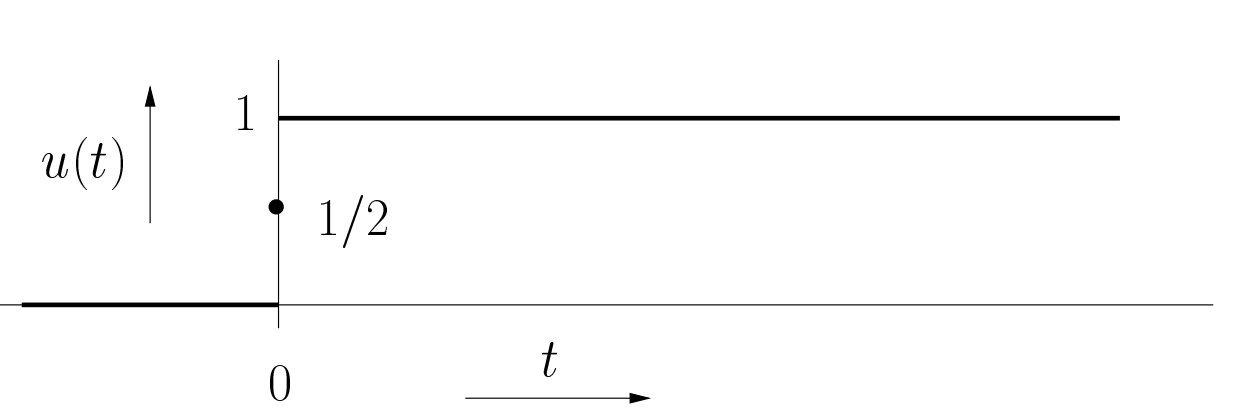
\includegraphics[width = 5cm]{include/Wichtige Funktionen/img/Sprungfunktion.png}
  \\ $H(t) = u(t) = \begin{cases}
      0 \textrm{ für }  t<0,                                                     \\
      [\frac{1}{2} \textrm{ für }  t = 0,] \textrm{ \tiny(machmal: 1 für $t=0$)} \\
      1 \textrm{ für }  t >0.
    \end{cases}   $
  \\
  \subsubsection*{Diracimpuls \tiny (auch Impuls-/Deltafunktion,-Distribution)}
  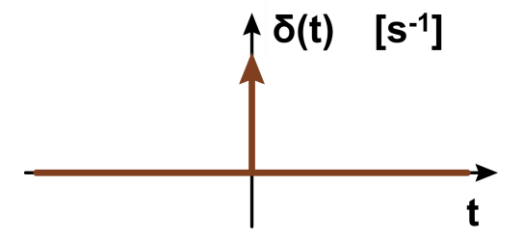
\includegraphics[width = 5cm]{include/Wichtige Funktionen/img/Impulsfunktion.png}
  \\ \footnotesize
  Unendlich kurzer, normierter Impuls mit unendlicher Amplitude.
  \\Eigenschaften:\\
  \resizebox{0.4\textwidth}{!}{%
    \begin{tabular}{ccc}
      \hline \rowcolor{TabularBackgroundColor}
      1.  & $\delta(-t) = \delta(t) $                                                                                            & gerade Funktion                        \\
      \hline
      2.  & $\delta(-t+t_0) = \delta(t-t_0)$                                                                                     & symmetrisch                            \\
      \hline \rowcolor{TabularBackgroundColor}
      3.  & $\delta(at)= \frac{1}{|a|}\delta(t)$                                                                                 & Skalierung                             \\
      \hline
      4.  & $\delta(\frac{t-t_0}{a}) = |a| \cdot \delta(t-t_0)$                                                                  & Skalierung und Verschiebung            \\
      \hline \rowcolor{TabularBackgroundColor}
      5.  & $\delta(t-t_0)f(t) = f(t_0)\delta(t-t_0)$                                                                            & Abtastung                              \\
      \hline
      6.  & $\int \limits _{-\infty} ^{\infty} \delta(t-t_0)f(t)dt = f(t_0)$                                                     & Siebungseigenschaft                    \\
      \hline \rowcolor{TabularBackgroundColor}
      7.  & $\int \limits _{-\infty} ^{\infty}  A\cdot \delta(t)dt = A$                                                          & Spezialfall Siebungseigenschaft        \\
      \hline
      8.  & $\delta(t-t_0) * f(t) = f(t-t_0)$                                                                                    & Faltung                                \\
      \hline \rowcolor{TabularBackgroundColor}
      9.  & $\delta(t-t_1) * \delta(t-t_2) = \delta(t-t_1-t_2)$                                                                  & Faltung                                \\
      \hline
      10. & $\delta(t) = \frac{du(t)}{dt}$                                                                                       & Ableitung Einheitssprung               \\
      \hline \rowcolor{TabularBackgroundColor}
      11. & $ \delta(t) = \lim _{\omega \to \infty} \frac{sin(\omega t)}{\pi t} $                                                & Definition                             \\
      \hline
      12. & $ \delta(t) = \lim _{\epsilon \to \infty} \frac{\epsilon}{\pi(t^2 + \epsilon^2)} $                                   & Definition                             \\
      \hline \rowcolor{TabularBackgroundColor}
      13. & $\delta(t) = \lim _{\epsilon \to 0} \frac{e^{-t^2/\epsilon}}{\sqrt{(\pi \epsilon)}} $                                & Definition                             \\
      \hline
      14. & $t^n \frac{d^n \delta(t)}{dt^n} = (-1)^n n! \delta(t)$                                                               & Ableitung                              \\
      \hline \rowcolor{TabularBackgroundColor}
      15. & $f(t) * \frac{d\delta(t-t_0)}{dt} = \frac{df(t-t_0)}{dt}$                                                            & Faltung mit Ableitung                  \\
      \hline
      16. & $\frac{d\delta(t)}{dt} = \frac{\delta(t)}{-t} = \lim _{\epsilon \to 0} \frac{-2\epsilon t}{\pi(t^2 + \epsilon^2)^2}$ & 1. Ableitung $\delta(t)$ = ungerade F. \\
      \hline
    \end{tabular}}
  \subsubsection*{Signumfunktion (Vorzeichenfunktion)}
  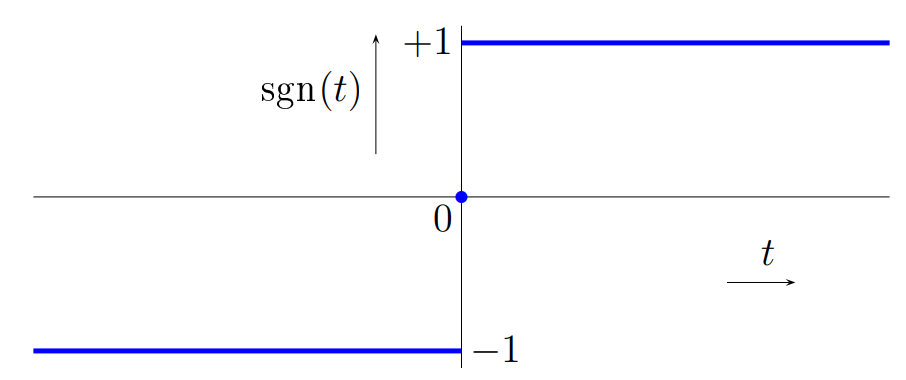
\includegraphics[width = 5cm]{include/Wichtige Funktionen/img/Signumfunktion.png}
  \footnotesize
  \\ $sgn(t) = \begin{cases}
      -1 \textrm{ für }  t<0,  \\
      0 \textrm{ für }  t = 0, \\
      1 \textrm{ für }  t >0.
    \end{cases}   $                                                          \\
  \subsubsection*{Rampenfunktion}
  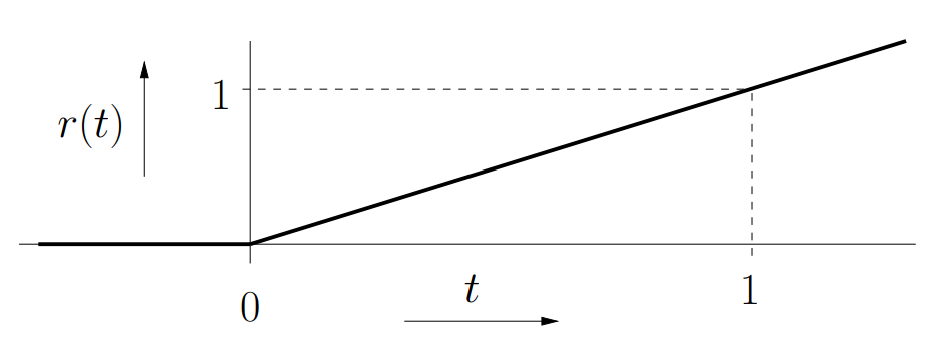
\includegraphics[width=5cm]{include/Wichtige Funktionen/img/Rampenfunktion.png}
  \footnotesize
  \\ $r(t) = \begin{cases}
      0 \textrm{ für } t \leq 0, \\
      t \textrm{ für } t > 0.
    \end{cases}$                                                          \\
  \subsubsection*{Rechteckimpuls}
  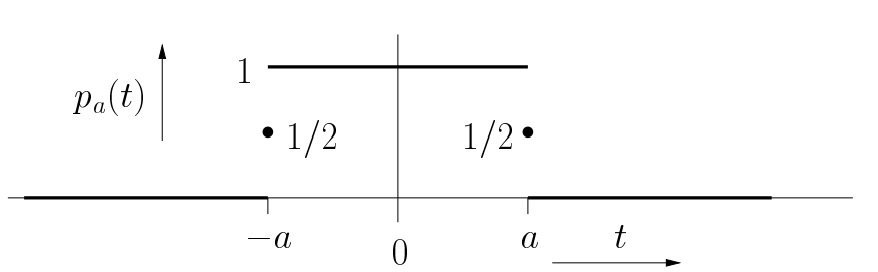
\includegraphics[width=5cm]{include/Wichtige Funktionen/img/Rechteckimpuls.png}
  \footnotesize
  \\ $p_a(t) = u(t+a)-u(t-a)= \begin{cases}
      1 \textrm{ für } |t| < a,           \\
      \frac{1}{2} \textrm{ für } |t| = a, \\
      0 \textrm{ für } |t| > a.
    \end{cases} $                               \\
  \subsubsection*{Dreieckimpuls}
  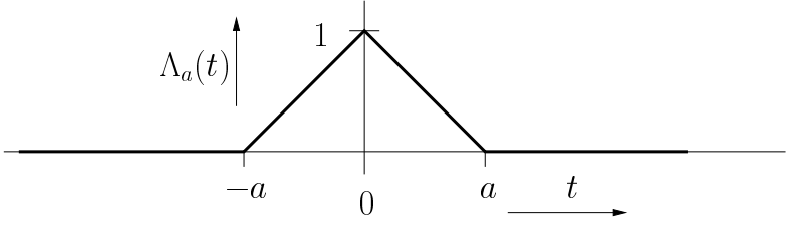
\includegraphics[width=5cm]{include/Wichtige Funktionen/img/Dreieckimpuls.png}
  \footnotesize
  \\ $\Lambda(t) = \begin{cases}
      1 - \frac{|t|}{a} \textrm{ für } |t| < a \\
      0 \textrm{ für } |t| \geq a
    \end{cases}$                                      \\
  \subsubsection*{Sinc-Funktion}
  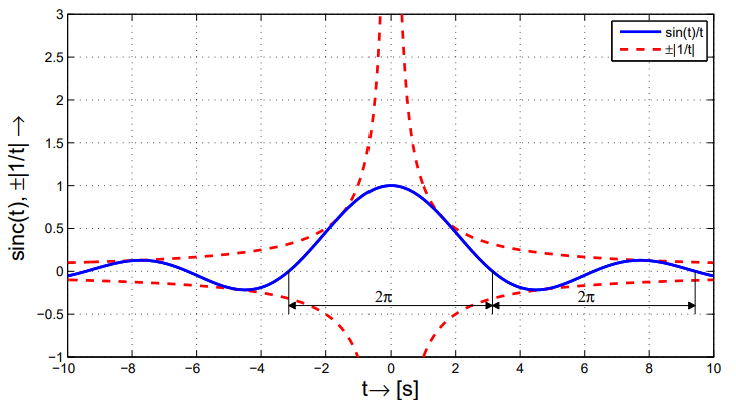
\includegraphics[width=5cm]{include/Wichtige Funktionen/img/SincFunktion.png}
  \footnotesize
  \\ $sinc(t) = \frac{sin(t)}{t} \forall t$                                                                                   \\
\end{multicols}
